

\subsection*{Homework Problems}

The following are some more involved problems for you to try, which might be assigned as homework.

\begin{questions}

\question Your ``friend'' has shown you a ``proof'' he wrote to show that $1 = 3$.  Here is the proof:

\begin{proof}
We want to show that $1 = 3$.  Of course we can do anything to one side of an equation as long as we also do it to the other side.  So subtract 2 from both sides.  This gives $-1 = 1$.  Now square both sides, to get $1 = 1$.  And we all agree this is true. Thus $1=3$.
\end{proof}

Carefully explain what is wrong with this proof using what we know about logic.  Hint: First identify the implication which follows from the proof.

\begin{solution}
In the proof we assume that $1=3$ and conclude that $1=1$.  So we have proved the implication
\[1=3 \imp 1=1\]
Note that we actually have a valid proof of this, and that the implication is true (for one thing, the ``if'' part is true, so the implication is automatically true).  However, what we really want is to converse of this, that $1=1 \imp 1=3$.  But as we know, the converse is not implied by the original implication (it better not be, otherwise we could conclude that 1 actually was 3).  

Another way to say this: we can never conclude anything about the ``if'' part of an implication, since the ``if'' part can be true or false even if the implication is true.
\end{solution}



\question Tommy Flanagan was telling you what he ate yesterday afternoon.  He tells you, ``I had either popcorn or raisins.  Also, if I had cucumber sandwiches, then I had soda.  But I didn't drink soda or tea.''  Of course you know that Tommy is the worlds worst liar, and everything he says is false.  What did Tommy eat?  

Justify your answer by writing all Tommy's statements using sentence variables ($P, Q, R, S, T$), taking their negations, and using these to deduce what Tommy actually ate.

\begin{solution}
Let $P$ be the statement, ``I had popcorn,'' $Q$ be the statement, ``I had cucumber sandwiches,'' $R$ be the statement, ``I had raisins,'' $S$ be, ``I had soda,'' and $T$ be, ``I had tea.''  Then the statements made by Tommy are:
\[P \vee R \qquad Q \imp S \qquad \neg(S \vee T)\]
We need the negation of all of these.  Thus what is true is:
\[\neg P \wedge \neg R \qquad Q \wedge \neg S \qquad S \vee T\]
From the first two statements we can conclude that Tommy did not eat popcorn, did not eat raisins, did eat cucumber sandwiches and did not drink soda.  From the last statement $S \vee T$ and the fact that we know $\neg S$ we can conclude $T$, so Tommy did drink tea.
\end{solution}


\question Use De Morgan's Laws, and any other logical equivalence facts you know to simplify the following statements.  Show all your steps.  Your final statements should have negations only appear directly next to the sentence variables or predicates ($P$, $Q$, $E(x)$, etc.), and no double negations.  It would be a good idea to use only conjunctions, disjunctions, and negations.
\begin{parts}
  \part $\neg((\neg P \wedge Q) \vee \neg(R \vee \neg S))$.
  \begin{solution}
    $\neg((\neg P \wedge Q) \vee \neg(R \vee \neg S))$\\
    $\neg(\neg P \wedge Q) \wedge \neg\neg(R \vee \neg S)$ by De Morgan's law.\\
    $\neg(\neg P \wedge Q) \wedge (R \vee \neg S)$ by double negation.\\
    $(\neg\neg P \vee \neg Q) \wedge (R \vee \neg S)$ by De Morgan's law.\\
    $(P \vee \neg Q) \wedge (R \vee \neg S)$ by double negation.
  \end{solution}

  \part $\neg((\neg P \imp \neg Q) \wedge (\neg Q \imp R))$ (careful with the implications).
  \begin{solution}
    We will need to convert the implications to disjunctions so we can apply De Morgan's law:
    
    $\neg((\neg P \imp \neg Q) \wedge (\neg Q \imp R))$\\
    $\neg((\neg \neg P \vee \neg Q) \wedge (\neg\neg Q \vee R))$ by implication/disjunction equivalence.\\
    $\neg((P \vee \neg Q) \wedge (Q \vee R))$ by double negation.\\
    $\neg(P \vee \neg Q) \vee \neg (Q \vee R)$ by De Morgan's law.\\
    $(\neg P \wedge \neg \neg Q) \vee (\neg Q \wedge \neg R)$ by De Morgan's law.\\
    $(\neg P \wedge Q) \vee (\neg Q \wedge \neg R)$ by double negation.
  \end{solution}


  \part $\neg \forall x \exists y ((E(x) \vee \neg O(y)) \imp \exists z (E(z) \wedge E(y)))$. Here, also put all the quantifiers ``out front.''
  \begin{solution}
  FIX
  \end{solution}
\end{parts}




\question Can you chain implications together?  That is, if $P \imp Q$ and $Q \imp R$, does that means the $P \imp R$?  Can you chain more implications together?  Let's find out:
\begin{parts}
  \part Prove that the following is a valid argument form:
  \begin{tabular}{rc}
    & $P \imp Q$ \\
    & $Q \imp R$ \\ \hline
    $\therefore$ & $P \imp R$
  \end{tabular}
  
  \begin{solution}
    Consider the truth table:
    
    \begin{tabular}{c|c|c||c|c|c}
      $P$ & $Q$ & $R$ & $P\imp Q$ & $Q \imp R$ & $P \imp R$ \\ \hline
      T   &  T  &  T  &     T     &      T     &      T \\
      T   &  T  &  F  &     T     &      F     &      F \\
      T   &  F  &  T  &     F     &      T     &      T \\
      T   &  F  &  F  &     F     &      T     &      F \\
      F   &  T  &  T  &     T     &      T     &      T \\
      F   &  T  &  F  &     T     &      F     &      T \\
      F   &  F  &  T  &     T     &      T     &      T \\
      F   &  F  &  F  &     T     &      T     &      T \\
    \end{tabular}
    Notice that both $P \imp Q$ and $Q \imp R$ are true in rows 1, 5, 7 and 8.  In each of these rows, $P \imp R$ is also true.  So whenever the premises are true, so in the conclusion.  Thus the argument form is valid.
  \end{solution}


\part Prove that the following is a valid argument form for any $n \ge 2$: 

\begin{tabular}{rc}
  & $P_1 \imp P_2$\\
  & $P_2 \imp P_3$ \\ 
  & $\vdots$ \\
  & $P_{n-1} \imp P_n$ \\ \hline
  $\therefore$ & $P_1 \imp P_n$.
\end{tabular}

I suggest you don't go through the trouble of writing out a $2^n$ row truth table.  Instead, you should use part (a) and mathematical induction.
\begin{solution}
Part (a) is the inductive case.  Now assume that the deduction rule holds going up to $P_k$.  That is, 

\begin{tabular}{rc}
  & $P_1 \imp P_2$\\
  & $P_2 \imp P_3$ \\ 
  & $\vdots$ \\
  & $P_{k-1} \imp P_k$ \\ \hline
  $\therefore$ & $P_1 \imp P_k$.
\end{tabular}

Now suppose we have

\begin{tabular}{rc}
  & $P_1 \imp P_2$\\
  & $P_2 \imp P_3$ \\ 
  & $\vdots$ \\
  & $P_{k-1} \imp P_k$ \\ 
  & $P_k \imp P_{k+1}$
\end{tabular}

From the first $k-1$ lines, we can conclude $P_1 \imp P_k$.  The combining this with the last line, we can conclude (using part (a) again):

\begin{tabular}{rc}
  & $P_1 \imp P_k$\\
  & $P_{k} \imp P_{k+1}$ \\ \hline
  $\therefore$ & $P_1 \imp P_{k+1}$.
\end{tabular}

So 

\begin{tabular}{rc}
  & $P_1 \imp P_2$\\
  & $P_2 \imp P_3$ \\ 
  & $\vdots$ \\
  & $P_{k-1} \imp P_k$ \\ 
  & $P_k \imp P_{k+1}$\\ \hline
  $\therefore$ & $P_1 \imp P_{k+1}$.  
\end{tabular}
\end{solution}

\end{parts}







\question  Consider the statement: $\forall x \forall y (x-y \ge 2 \imp \exists z (y < z \wedge z < x))$.
\begin{parts}
\part Explain what this statement says in words.  Is the statement true?
\begin{solution}
 The strictest translation: For all $x$ and for all $y$, if $x - y$ is at least 2, then there is a number $z$ which is larger than $y$ and less than $x$. 
 
 Alternatively, given any two numbers $x$ and $y$, if $x$ is at least two larger than $y$, then there is a number between them.  Or even more loose: For any numbers at least two apart, there is a number between them.
 
 The statement is true! (As long as we are looking at the integers, or real numbers.  If we considered our universe of discourse to be the even numbers say, then the statement would be false.)
\end{solution}

\part State the contrapositive of the original statement.  Do so both in words and in symbols.
\begin{solution}
 The contrapositive: for all $x$ and $y$, if there is no number $z$ larger than $y$ and smaller than $x$, then $x - y < 2$.  Or if you simplify, for all $x$ and $y$, if every $z$ is either not greater than $y$ or not less than $x$, then $x - y$ is less than $2$.
 
 \[\forall x \forall y (\forall z (y \ge z \vee z \ge x) \imp x-y < 2)\]
\end{solution}

\part State the converse of the original statement.  Is the converse true?
\begin{solution}
 The converse is, for all $x$ and for all $y$, if there is some $z$ greater than $y$ and less than $x$, then $x-y \ge 2$.  Or in symbols,
 \[\forall x \forall y (\exists z (y < z \wedge z < x) \imp x-y \ge 2)\]
 The converse is true, as long as we consider only the integers, but false if we consider the real numbers (or rationals).
\end{solution}

\part State the negation of the original statement.  Do so both in words and in symbols (simplifying as much as possible).
\begin{solution}
 The negation: there are numbers $x$ and $y$ such that $x - y$ is at least 2, but for all $z$, either $z$ is not larger than $y$ or not less than $x$.
 
 \[\exists x \exists y (x - y \ge 2 \wedge \forall z (y \ge z \vee z \ge x))\]
\end{solution}

\end{parts}


\question Suppose that you would like to prove the following implication: 
\begin{center}
``For all numbers $n$, if $n$ is prime then $n$ is solitary". 
\end{center}
Write out the beginning and end of the argument if you were to prove the statement, 
\begin{parts}
\part Directly
\begin{solution}
To solve the above statement using a direct proof we would need to start by  assuming that $n$ is a prime number then using logic, logic, logic,... we could conclude that $n$ is solitary.
\end{solution}
\part By contrapositive
\begin{solution}
To solve by contrapositive: Assume $n$ is not solitary (logic, logic, logic...) and conclude that $n$ is not prime.
\end{solution}
\part By contradiction
\begin{solution}
To solve using a proof by contradiction: Assume that $n$ is prime and that $n$ is not solitary (logic, logic, logic...) then either $n$ is not prime or $n$ is solitary (you need to contradict one of your assumptions). Therefore, if $n$ is prime then $n$ is solitary.
\end{solution}
\end{parts}
You do not need to provide details for the proofs (since you do not know what solitary means). However, make sure that you provide the first few and last few lines of the proofs so that we can see that logical structure you would follow.



\question A standard deck of 52 cards consists of 4 suites (hearts, diamonds, spades and clubs) each containing 13 different values (Ace, 2, 3, \ldots, 10, J, Q, K).  If you draw some number of cards at random you might or might not have a pair (two cards with the same value) or three cards all of the same suit.  However, if you draw enough cards, you will be guaranteed to have these.  For each of the following, find the smallest number of cards you would need to draw to be guaranteed having the specified cards.  Prove your answers.
\begin{parts}

\part Three of a kind (for example, three 7's).
\begin{solution}
The worst case scenario that could happen before you drew three of a kind would be $26$ because that would mean that you have drawn exactly $2$ of each card, Ace through King. Thus, as soon as you draw the $27$th card, you will have three of a kind.
\end{solution}

\part A flush of five cards (for example, five hearts). 
\begin{solution}
Okay, let's think about the worst case scenario again. If I drew 4 of every suit (hearts, spades, diamonds, and clubs) then I would have 16 cards and not yet have a 5 card flush. However, as soon as I draw the $17$th card, I have 5 cards of the same suit no matter which suit I draw.
\end{solution}

\part Three cards that are either all the same suit or all different suits.
\begin{solution}
You must pick 5 cards.  If you picked just 4, you could have two hearts and two spades.  However, given any 5 cards, we can be sure that at least two of them will be the same suit, say hearts.  Of the remaining three cards, if any of them are also a heart, we will have three hearts.  If not,  there are two cases to consider.  Either all three cards will be of the same suit (in which case we would have three cards of the same suit) or else two suits will be present among the three cards.  But those two other suits are not hearts, so those two cards plus one of the hearts will form a set of three cards of all different suits. 
\end{solution}
\end{parts}



\question Suppose you are at a party with 19 of your closest friends (so including you, there are 20 people there).  Explain why there must be least two people at the party who are friends with the same number of people at the party.  Assume friendship is always reciprocated.

\begin{solution}
  Suppose this was not the case.  That is, suppose everyone at the party had a {\em different} number of friends.  What could these numbers be.  The would have to be less than 20, so each number from 0 to 19 (that's 20 numbers) must be used exactly once.  But this is impossible. If someone is friends with 19 people, then she is friends with everyone, including the person who is supposedly friends with 0 people.
  
  What this says is that in any simple graph with 20 vertices, there must be at least two vertices which have the same degree.
\end{solution}


\question Suppose you have an $n\times n$ chessboard but your dog has eaten one of the corner squares. Can you still cover the remaining squares with dominoes? What needs to be true about $n$? Give necessary and sufficient conditions (that is, say exactly which values of $n$ work and which do not work). Prove your answers.

\begin{center}
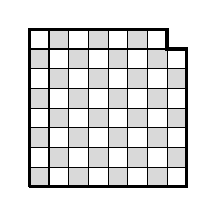
\begin{tikzpicture}[scale=.25]
\foreach \x in {0,2,...,6}{
	\foreach \y in {0,2,...,6}{
\draw[fill=white!85!black] (\x,\y) rectangle (\x+1, \y+1) rectangle (\x+2,\y+2);
}}
\draw (0,0) grid (8,8);
\draw[white, fill=white] (7,7) rectangle (8,8);
\draw[very thick] (0,0) -- (8,0) --(8,7) -- (7,7) -- (7,8) -- (0,8) -- (0,0);
\end{tikzpicture}
\end{center}
\begin{solution}
Yes, we can in fact still cover the chessboard with dominoes but only if $n$ is odd. So, my claim is that if $n$ is odd, then I can cover the above chessboard. 
%But does this claim hold in the reverse? If I have covered the above chessboard then $n$ is odd. Yes, it does in fact work. Now, I need to prove that the above chessboard is covered with dominoes if and only if $n$ is odd. 
To prove this, I am going to first notice that if I take away the column and row attached to the missing square, I have created an $n-1\times n-1$ chessboard where $n-1$ is even. By the proof in class, we have shown that that can be completely covered with dominoes. So, now I just need to worry about the row and column I took away. Since $n$ is odd, I know that the row and column are even and thus can be covered by dominoes lined up head to tail. Thus, I have shown that if $n$ is odd then I can completely cover an $n\times n$ chessboard if $n$ is odd.
\end{solution}

\question Bonus: What if your $n\times n$ chessboard is missing two opposite corners?  Prove that no matter what $n$ is, you will not be able to cover the remaining squares with dominoes. 

\begin{center}
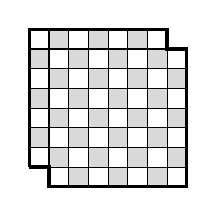
\begin{tikzpicture}[scale=.25]
\foreach \x in {0,2,...,6}{
	\foreach \y in {0,2,...,6}{
\draw[fill=white!85!black] (\x,\y) rectangle (\x+1, \y+1) rectangle (\x+2,\y+2);
}}
\draw (0,0) grid (8,8);
\draw[white, fill=white] (7,7) rectangle (8,8) (0,0) rectangle (1,1);
\draw[very thick] (0,1) -- (1,1) -- (1,0) -- (8,0) --(8,7) -- (7,7) -- (7,8) -- (0,8) -- (0,1);
\end{tikzpicture}
\end{center}

\begin{solution}
First notice that both removed squares have identical color. So their removal leaves us with $\frac{n}{2}$ squares of one color and $\frac{n-2}{2}$ squares of the other color. Since a domino always covers one black and one white squares, the remaining squares cannot be tiled.
\end{solution}


 
 
\end{questions}


